\chapter{Methods}\label{chap:methods}
\thispagestyle{fancy} %Resets custom page number location on first chapter page

Misalignments produce aberrations, but phase retrieval recovers only the wavefront; inferring the positions of the telescope optics requires a second, model-based step, such as the linear multi-field inversion used during JWST commissioning (Chapter~\ref{sec:intro}). In this work, we instead use a ray-trace model of the telescope to infer mirror misalignments directly from PSF observations.

To perform misalignment inference, we construct a pipeline (Figure~\ref{fig:block}) that does the following:
\begin{enumerate}
    \item Build a parametric telescope in Optiland~\citep{Harrison_Optiland_2026} and propagate monochromatic light to generate a synthetic PSF.
    \item Project PSF onto a basis.
    \item Model observations as multivariate Gaussians in coefficient space with field-specific covariances $\boldsymbol{\Sigma}_f$ from Monte Carlo calibration.
    \item Explore the posterior with Nautilus~\citep{Lange2023}, and then refine a point estimate with differential evolution.
    \item Validate by comparing nominal and residual-alignment systems in PSF and OPD space.
\end{enumerate}

\begin{figure*}
    \centering
    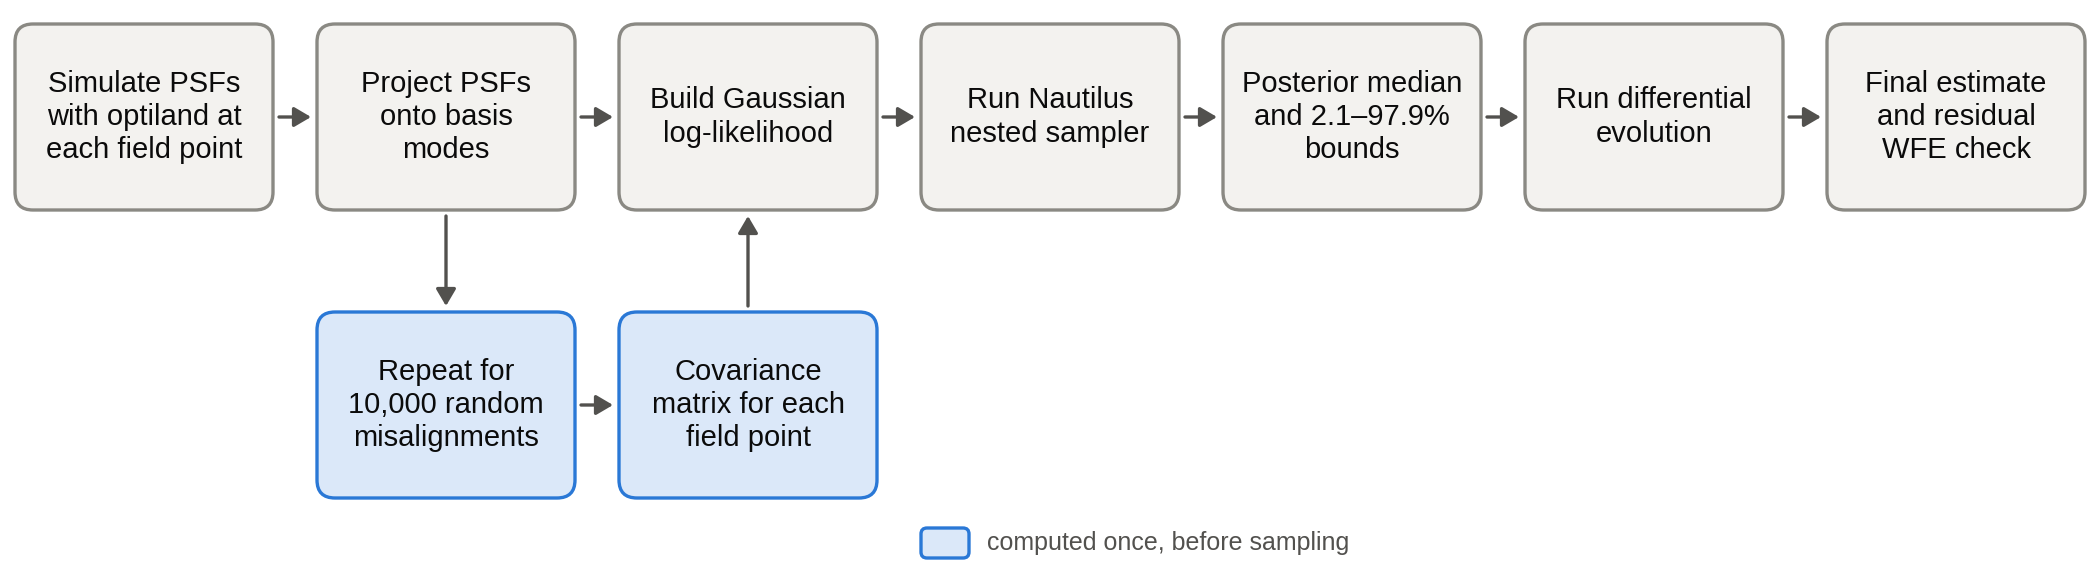
\includegraphics[width=\textwidth]{figures/block_diagram.png}
    \caption{Inference pipeline: Optiland forward model, basis-coefficient feature extraction, multivariate Gaussian likelihood, Nautilus nested sampling, and differential-evolution refinement with PSF/OPD validation.}
    \label{fig:block}
\end{figure*}

\section{Raytracing}\label{sec:raytracing}
Both telescope models are built and traced in Optiland~\citep{Harrison_Optiland_2026} (version 0.6.0; see Section~\ref{sec:software}), an open-source Python ray tracer, using its NumPy backend in double precision. Each mirror is a conic surface with sag
\begin{equation}
z(r) = \frac{r^2/R}{1+\sqrt{1-(1+k)\,r^2/R^2}},
\end{equation}
where $R$ is the vertex radius of curvature, $k$ is the conic constant and $r$ is the radial distance from the vertex. Real rays are traced sequentially from an object at infinity and intersect each surface exactly rather than through a paraxial approximation, so the forward model contains every order of aberration that a misalignment introduces. Lengths are in millimeters and wavelengths in micrometers. Table~\ref{tab:prescriptions} lists both prescriptions.

\begin{table}
\centering
\caption{Optical prescriptions of the two telescope models. Vertex positions $z$ are along the optical axis in the fixed laboratory frame used to place each surface.}
\label{tab:prescriptions}
\begin{tabular}{lllll}
\hline
Model & Surface & $R$ (mm) & $k$ & $z$ (mm) \\
\hline
Hubble & Primary (stop) & $-11040.02286$ & $-1.001152$ & $4910.01016$ \\
       & Secondary      & $-1349.31166$  & $-1.483014$ & $0$ \\
       & Image          & $-635.38227$   & ---         & $6365.20955$ \\
\hline
TMA    & M1 (stop)      & $-16256$       & $-0.995357$ & $0$ \\
       & M2             & $-1660.575$    & $-1.566503$ & $-7400.005$ \\
       & M3             & $-1830.5174$   & $-0.718069$ & $49.965$ \\
       & M4 (fold)      & $\infty$       & ---         & $-983.655$ \\
       & Image          & $\infty$       & ---         & $236.685$ \\
\hline
\end{tabular}
\end{table}

\subsection{Telescope models}
The Hubble model is a Ritchey--Chr{\'e}tien telescope with a 2400\,mm entrance pupil. The primary is the aperture stop and carries a physical mask: an annulus between radii of 384 and 1200\,mm, two orthogonal spider vanes 38\,mm wide, and three circular pads of 75\,mm radius centered 1000\,mm from the axis. The secondary sits 4910.01\,mm in front of the primary and the curved image surface lies 6365.21\,mm behind the secondary, giving a working f-number of 24.0. Field angles extend to $0.038^{\circ}$.

The TMA follows the design of \citet{PearlTMA}. Three powered conic mirrors form the image, and a flat fourth mirror folds the beam onto the detector, which is why the Optiland prescription has four mirrors. The entrance pupil is circular with a diameter of 6471.26\,mm, the primary is the stop, and the working f-number is 15.1. The prescription defines field angles of $0.055^{\circ}$, $0.17^{\circ}$ and $0.285^{\circ}$ along $y$. Normalized field coordinates are relative to $0.285^{\circ}$, so the near-axis field $(0,0.5965)$ used in the likelihood corresponds to $0.17^{\circ}$.

\subsection{Applying misalignments}
Rather than chaining surfaces through sequential thicknesses, every surface is placed in absolute coordinates: its vertex position $(x,y,z)$ and rotations $(r_x,r_y)$ are given in a fixed laboratory frame. A rigid-body misalignment of a mirror then changes only that mirror's coordinates. Decenters add to its $x$ and $y$, despace adds to its $z$, and tilts rotate it about its own vertex. All other surfaces, including the image surface, stay where they are, so moving the secondary does not drag the downstream optics or the detector with it, as it would if a despace were entered as a change in thickness. Misalignments are specified in micrometers and degrees and converted to millimeters and radians before tracing. The Hubble model perturbs only the secondary ($sdx$, $sdy$, $sdz$, $stx$, $sty$). The TMA perturbs the primary and the secondary ($pdx$, $pdy$, $pdz$, $ptx$, $pty$ and $sdx$, $sdy$, $sdz$, $stx$, $sty$), while M3, the fold mirror and the detector stay fixed.

\subsection{PSF computation}
PSFs are computed with Optiland's \bashinline{MMDFTPSF}. For a given field and wavelength it traces a uniform square grid of rays across the entrance pupil and computes the optical path difference $W$ of each ray, in waves, at the exit pupil relative to a reference sphere centered on the chief ray's image point. Each PSF is therefore centered on the chief ray: a misalignment that moves the whole image, and the chief ray with it, does not move the PSF within the frame. Tilt relative to the reference sphere is retained, so displacements of the light relative to the chief ray, such as the centroid shift produced by coma, do appear. The absolute position of the image on the detector is not used (Section~\ref{sec:noise_moves}). The complex pupil function is
\begin{equation}
P(x,y) = A(x,y)\,\exp\!\left[-2\pi i\,W(x,y)\right],
\end{equation}
where the amplitude $A$ follows from the transmitted ray intensity and is zero for rays blocked by the aperture mask. The focal-plane field is computed with a matrix-triple-product discrete Fourier transform~\citep{Soummer2007}, $E = L\,P\,R$, in which the matrices $L$ and $R$ set the image sampling independently of the pupil grid, and the PSF is $|E|^2$. Optiland scales the PSF so that a diffraction-limited system with the same aperture has a peak of 100. The peak of each PSF is therefore 100 times its Strehl ratio, and the noise level $\sigma=0.01$ used for the observations of both models (Sections~\ref{sec:hubble} and~\ref{sec:pearl}) is 0.01\% of the ideal peak.

The \bashinline{num_rays} argument $N$ sets both samplings, following the OpticStudio convention. The pupil is sampled with $n_{\mathrm{p}}=\lfloor 32\cdot 2^{(\log_2 N-5)/2}\rfloor$ rays across its diameter, the image grid is $2N\times 2N$ pixels, and the pixel pitch is chosen so that the grid spans $(n_{\mathrm{p}}-1)\,\lambda F_\#$. Only a central patch of the image is kept for the basis projection. Table~\ref{tab:psf_sampling} lists the resulting values for both models. The PSFs are monochromatic and contain no detector effects such as pixel integration, jitter or read noise.

\begin{table}
\centering
\caption{PSF sampling for the two models.}
\label{tab:psf_sampling}
\begin{tabular}{lll}
\hline
 & Hubble & TMA \\
\hline
Wavelength & $0.55\,\mu$m & $0.65\,\mu$m \\
Working f-number $F_\#$ & 24.0 & 15.1 \\
\bashinline{num_rays} $N$ & 128 & 512 \\
Pupil samples & $64\times64$ & $128\times128$ \\
Image grid & $256\times256$ & $1024\times1024$ \\
Pixel pitch & $3.25\,\mu$m & $1.21\,\mu$m \\
Pixels per $\lambda F_\#$ & 4.06 & 8.06 \\
Retained patch & $64\times64$ ($15.8\,\lambda F_\#$) & $256\times256$ ($31.8\,\lambda F_\#$) \\
\hline
\end{tabular}
\end{table}

\subsection{Wavefront error}
Recovered alignments are validated by comparing optical path difference maps. Optiland's \bashinline{OPD} traces a hexapolar ray pattern of 15 rings at the requested field, computes the OPD in waves relative to the same chief-ray reference sphere, and interpolates it onto a $256\times256$ pupil grid. The RMS wavefront error quoted in Chapters~\ref{chap:hubble} and~\ref{chap:tma} is the standard deviation, over the pupil, of the difference between the OPD map of the nominal design and that of the residual system with misalignments $\boldsymbol{\theta}_{\mathrm{true}}-\mathbf{c}$. Taking the standard deviation removes piston; tilt is retained.

\section{Nested sampling}\label{sec:nested}

\subsection{Bayesian inference}
We treat the misalignment $\boldsymbol{\theta}$ as uncertain and describe what the observations imply about it with Bayes' theorem,
\begin{equation}
P(\boldsymbol{\theta}\mid D) = \frac{\mathcal{L}(\boldsymbol{\theta})\,\pi(\boldsymbol{\theta})}{\mathcal{Z}},\qquad
\mathcal{Z} = \int \mathcal{L}(\boldsymbol{\theta})\,\pi(\boldsymbol{\theta})\,\mathrm{d}\boldsymbol{\theta},
\label{eq:bayes}
\end{equation}
where $D$ denotes the observed coefficients, $\mathcal{L}(\boldsymbol{\theta})=P(D\mid\boldsymbol{\theta})$ is the likelihood, $\pi(\boldsymbol{\theta})$ is the prior, and the evidence $\mathcal{Z}$ normalizes the posterior. The posterior says more than a single best fit. Its marginals show how well each parameter is constrained, and correlations between parameters reveal combinations of mirror motions that produce nearly the same PSFs (Chapters~\ref{chap:hubble} and~\ref{chap:tma}). The evidence is the quantity used to compare models, for example telescope models with different sets of free parameters; we report it for each run but do not use it for model selection here.

With five or ten parameters, the posterior cannot be mapped on a grid. A misaligned telescope can also produce a likelihood surface with separated maxima or long curved ridges, which are difficult for local optimizers and slow the mixing of Markov chain Monte Carlo samplers. Nested sampling~\citep{Skilling2006} was designed to compute $\mathcal{Z}$ for such problems, and it yields posterior samples as a by-product.

\subsection{The nested sampling algorithm}
Nested sampling turns the multidimensional evidence integral into a one-dimensional one. The prior volume enclosed by the likelihood contour $\lambda$,
\begin{equation}
X(\lambda) = \int_{\mathcal{L}(\boldsymbol{\theta})>\lambda} \pi(\boldsymbol{\theta})\,\mathrm{d}\boldsymbol{\theta},
\end{equation}
falls from 1 to 0 as $\lambda$ rises from the lowest to the highest likelihood. Writing $\mathcal{L}(X)$ for the inverse of this function, the evidence becomes
\begin{equation}
\mathcal{Z} = \int_0^1 \mathcal{L}(X)\,\mathrm{d}X.
\end{equation}
The algorithm (Algorithm~\ref{alg:cap}) evaluates this integral with a set of $K$ live points drawn from the prior. At each iteration $i$, the live point with the lowest likelihood, $\mathcal{L}_i$, is recorded as a dead point and replaced by a new point drawn from the prior subject to $\mathcal{L}>\mathcal{L}_i$. The live points therefore always sample the prior inside a shrinking likelihood contour. At each step the enclosed volume shrinks by a factor $t_i$ distributed as the largest of $K$ uniform random numbers, with $\langle\ln t_i\rangle=-1/K$, so after $i$ iterations $X_i\approx e^{-i/K}$. The evidence is then the sum
\begin{equation}
\mathcal{Z} \approx \sum_i \mathcal{L}_i\,w_i,\qquad w_i = X_{i-1}-X_i,
\end{equation}
and each dead point becomes a posterior sample with weight $p_i=\mathcal{L}_i w_i/\mathcal{Z}$. The run stops once the live points can add only a small fraction of the evidence, and the remaining live points are then added with the final volume divided equally among them. The statistical uncertainty of $\ln\mathcal{Z}$ is approximately $\sqrt{H/K}$, where
\begin{equation}
H = \int P(\boldsymbol{\theta}\mid D)\,\ln\frac{P(\boldsymbol{\theta}\mid D)}{\pi(\boldsymbol{\theta})}\,\mathrm{d}\boldsymbol{\theta}
\end{equation}
is the information gained from prior to posterior; the number of iterations needed grows as $KH$.

\begin{algorithm}
\caption{Nested sampling}\label{alg:cap}
\begin{algorithmic}
\State Draw $K$ live points from the prior; set $X_0=1$, $\mathcal{Z}=0$ and $i=0$
\While{the live points can still add more than a small fraction of $\mathcal{Z}$}
\State $i \gets i+1$
\State Find the live point with the lowest likelihood, $\mathcal{L}_i$
\State Set $X_i=e^{-i/K}$ and $w_i=X_{i-1}-X_i$, and add $\mathcal{L}_i w_i$ to $\mathcal{Z}$
\State Move that point to the dead points with weight $\mathcal{L}_i w_i$
\State Replace it with a new point drawn from the prior subject to $\mathcal{L}>\mathcal{L}_i$
\EndWhile
\State Add the remaining live points to $\mathcal{Z}$ and to the dead points, each with $w=X_i/K$
\State Divide all weights by $\mathcal{Z}$ to obtain the posterior samples
\end{algorithmic}
\end{algorithm}

The difficult step is drawing a new point from the prior inside the current contour. Drawing from the whole prior and rejecting points below the threshold succeeds with probability $X_i$, which falls exponentially with $i$. Practical samplers therefore restrict the draws to a region that encloses the live points, for example a union of ellipsoids fitted to them, and reject only the draws inside that region that fall below the threshold~\citep{Feroz_2019}.

\subsection{Importance nested sampling with Nautilus}
Classic nested sampling keeps only the dead points; the many likelihood evaluations rejected while searching for each new live point are discarded. Importance nested sampling~\citep{Feroz_2019} instead keeps every point at which the likelihood was evaluated and weights it by the ratio of the posterior to the density from which it was drawn. We use \texttt{Nautilus}~\citep{Lange2023}, version 1.0.6, which builds on this idea and replaces the ellipsoidal sampling regions with bounds learned by neural networks.

Nautilus constructs a sequence of nested bounds in the unit cube $[0,1]^d$ on which the prior is defined (Section~\ref{sec:prior_like}). The first bound is the whole cube. Each later bound is built from all points evaluated so far. Its likelihood threshold is the $n_{\mathrm{live}}$-th highest likelihood among them; the points above the threshold are enclosed by one or more ellipsoids; and within each ellipsoid an ensemble of neural networks is trained to predict the rank of a point's likelihood. A point belongs to the bound if it lies inside an ellipsoid and the networks predict a likelihood above the threshold, which lets the bound follow curved or elongated contours more closely than an ellipsoid alone. A new bound is kept only if its volume is smaller than that of the previous one. The region inside one bound but outside all later bounds is a shell, and new points are drawn uniformly within a shell.

Sampling proceeds in two phases. In the exploration phase, Nautilus draws points in the innermost shell and adds a new bound after every $n_{\mathrm{live}}$ new points above the current threshold (or every $10\,n_{\mathrm{live}}$ likelihood calls), until the $n_{\mathrm{live}}$ highest-likelihood points hold less than a fraction $f_{\mathrm{live}}$ of the estimated evidence. In the sampling phase, it adds batches of points to the shells that limit the precision of the weighted posterior, until the effective sample size
\begin{equation}
N_{\mathrm{eff}} = \frac{\bigl(\sum_k w_k\bigr)^2}{\sum_k w_k^2}
\end{equation}
reaches a target. A point $\boldsymbol{\theta}_k$ in shell $j$ receives the weight $w_k\propto\mathcal{L}(\boldsymbol{\theta}_k)\,V_j/n_j$, where $V_j$ is the estimated volume of the shell and $n_j$ is the number of points in it. The evidence is $\mathcal{Z}=\sum_j V_j\,\bar{\mathcal{L}}_j$, the sum over shells of volume times mean likelihood. Because every evaluated point is used, $N_{\mathrm{eff}}$ is a substantial fraction of the number of likelihood calls.

Both runs used the default settings of Nautilus 1.0.6 (Table~\ref{tab:nautilus}) without a fixed random seed, so repeated runs give statistically equivalent but not identical results. The points drawn during the exploration phase are kept, which is also the default; the Nautilus documentation notes that discarding them is required for a fully unbiased posterior and evidence, at the cost of fewer samples.

\begin{table}
\centering
\caption{Nautilus settings and run statistics.}
\label{tab:nautilus}
\begin{tabular}{lll}
\hline
 & Hubble & TMA \\
\hline
Parameters $d$ & 5 & 10 \\
Live points $n_{\mathrm{live}}$ & 2000 & 2000 \\
Neural networks per bound & 4 & 4 \\
Exploration stops at $f_{\mathrm{live}}$ & 0.01 & 0.01 \\
Target $N_{\mathrm{eff}}$ & $10^4$ & $10^4$ \\
Bounds built & 17 & 38 \\
Ellipsoids in the final bound & 1 & 1 \\
Likelihood evaluations & 44\,000 & 93\,200 \\
Final $N_{\mathrm{eff}}$ & 14\,250 & 20\,373 \\
$N_{\mathrm{eff}}$ per likelihood evaluation & 0.32 & 0.22 \\
$\ln\mathcal{Z}$ & $+62.3$ & $+475.5$ \\
\hline
\end{tabular}
\end{table}

\subsection{Prior and likelihood}\label{sec:prior_like}
Nautilus samples the unit cube, and a prior transform maps $\mathbf{u}\in[0,1]^d$ to the physical parameters. Both studies use independent uniform priors, $\theta_k=a_k(2u_k-1)$, a box of half-width $a_k$ centered on the nominal position; the half-widths are given in Sections~\ref{sec:hubble} and~\ref{sec:pearl}. The function passed to the sampler returns $\ln\mathcal{L}(\boldsymbol{\theta})$ only, since the prior density is uniform inside the box and zero outside. The Hubble transform also rounds each parameter to two decimal places, quantizing translations to $0.01\,\mu\mathrm{m}$ and tilts to $0.01^{\circ}$. Within the $\pm0.167^{\circ}$ prior, each tilt can therefore take only 35 values, which produces the striped tilt panels of Figure~\ref{fig:hubble_corner}. The TMA transform does not round.

The observations enter through the basis coefficients. At each field $f\in\mathcal{F}$, the coefficients $\mathbf{c}_f(\boldsymbol{\theta})$ predicted by the forward model are compared with the observed coefficients $\mathbf{c}_{f,\mathrm{obs}}$ through a multivariate Gaussian, and the log-likelihood sums the fields, treating them as independent. For the TMA, $\mathcal{F} = \{(0,0.5965),\allowbreak(1,0),\allowbreak(0,1),\allowbreak(1,1),\allowbreak(0,-1),\allowbreak(-1,0),\allowbreak(1,-1),\allowbreak(-1,1),\allowbreak(-1,-1),\allowbreak(0.5,0.5)\}$, where the near-axis field $(0,0.5965)$ is used in place of $(0,0)$; the Hubble field set is given in Section~\ref{sec:hubble}. The log-likelihood is
\begin{equation}
\begin{split}
\ln \mathcal{L}(\boldsymbol{\theta})
= \sum_{f \in \mathcal{F}} \Bigl\{
&-\frac{1}{2}
\left[\mathbf{c}_f(\boldsymbol{\theta}) - \mathbf{c}_{f,\mathrm{obs}}\right]^{\!\top}
\boldsymbol{\Sigma}_f^{-1}
\left[\mathbf{c}_f(\boldsymbol{\theta}) - \mathbf{c}_{f,\mathrm{obs}}\right] \\
&-\frac{N_z}{2}\ln(2\pi)
-\frac{1}{2}\ln\det\boldsymbol{\Sigma}_f
\Bigr\}
\end{split}
\label{eq:loglike}
\end{equation}
where $N_z$ is the number of retained modes (15 for Hubble, 11 for the TMA) and $\boldsymbol{\Sigma}_f$ is the covariance at field $f$. Each $\boldsymbol{\Sigma}_f$ is estimated once, before sampling, from $10^4$ noise-free forward-model evaluations at misalignments drawn from zero-mean Gaussians, whose widths are given in Sections~\ref{sec:hubble} and~\ref{sec:pearl}. It therefore describes how much the coefficients vary across plausible misalignments, not the measurement noise, which is far smaller (Chapter~\ref{chap:noise}). Because $\boldsymbol{\Sigma}_f$ does not depend on $\boldsymbol{\theta}$, the last two terms of equation~(\ref{eq:loglike}) are constant. They do not affect the posterior, but they set the value of $\ln\mathcal{Z}$, and they are included in the values of Table~\ref{tab:nautilus}.

\subsection{Using the posterior}
Nautilus returns the evaluated points together with their weights. The corner plots (Figures~\ref{fig:hubble_corner} and~\ref{fig:pearl_corner}) show the one- and two-dimensional marginals of these weighted samples, and their panel titles give the weighted median and the 16th--84th percentile range of each parameter. Nautilus stores the points shell by shell, from the unit cube inward, so the final 100 samples are the last points stored in the innermost, highest-likelihood shell. Within one shell every point has the same volume factor, so the weights of these samples are proportional to their likelihoods. They provide the starting point and the bounds for differential evolution (Section~\ref{sec:de}).

\section{Differential evolution}\label{sec:de}

\subsection{Why a second stage}
The nested-sampling posterior is broad. Its width is set by the calibration covariances $\boldsymbol{\Sigma}_f$, which describe the spread of the coefficients across the prior rather than the measurement noise (Chapter~\ref{chap:noise}), and some parameters remain nearly unconstrained along degenerate directions. To obtain a precise alignment estimate, we follow nested sampling with a direct minimization of the coefficient residuals,
\begin{equation}
S(\boldsymbol{\theta}) = \sum_{f\in\mathcal{F}}\sum_{k=1}^{N_z}\left[c_{f,k}(\boldsymbol{\theta}) - c_{f,k,\mathrm{obs}}\right]^2,
\label{eq:de_cost}
\end{equation}
the unweighted sum of squared differences between the forward-model and observed coefficients over all fields. Without noise, $S$ vanishes at the true alignment; with noise, its minimum is offset from the truth by an amount set by the noise (Section~\ref{sec:noise_de}). $S$ does not use $\boldsymbol{\Sigma}_f$, so the estimate does not depend on the calibration. The cost surface inherits the structure of the likelihood: it can have several local minima and long, flat valleys along degenerate combinations of mirror motions, where a gradient-based optimizer started from a single point can stall. We therefore use differential evolution (DE), a population-based global optimizer introduced by \citet{StornPrice1997}, as implemented in \bashinline{scipy.optimize.differential_evolution}~\citep{Virtanen2020}. DE needs only evaluations of $S$, not its gradient, which suits a ray-trace forward model whose derivatives are not available analytically.

\subsection{The algorithm}
DE evolves a population of $P$ candidate vectors inside box bounds (Algorithm~\ref{alg:de}). SciPy sets $P$ to a multiple, \bashinline{popsize}, of the number of parameters $d$; with the default \bashinline{popsize=15}, the population has 75 members for Hubble and 150 for the TMA. Internally, each member is stored in coordinates scaled to $[0,1]$ across the bounds, so mutation steps are proportional to the bound widths. The population is initialized by Latin hypercube sampling of the bounds, which spreads the members evenly along every parameter, and the starting point $\mathbf{x}_0$ from nested sampling replaces the first member.

Each generation then visits every member $\boldsymbol{\theta}_i$ in turn:
\begin{enumerate}
    \item \textbf{Mutation.} A mutant vector is formed from the current best member and the difference of two other members chosen at random,
    \begin{equation}
    \mathbf{v}_i = \boldsymbol{\theta}_{\mathrm{best}} + F\,(\boldsymbol{\theta}_{r_1} - \boldsymbol{\theta}_{r_2}).
    \end{equation}
    This is the \bashinline{best1} strategy. The difference vector adapts the step size to the spread of the population: steps are large while the members are scattered and shrink as they converge. The mutation factor $F$ is redrawn uniformly from $[0.5,1)$ at every generation, a variant known as dithering that can speed up convergence.
    \item \textbf{Crossover.} A trial vector $\mathbf{u}_i$ takes each parameter from $\mathbf{v}_i$ with probability $C_r=0.7$ and otherwise keeps it from $\boldsymbol{\theta}_i$; one randomly chosen parameter always comes from $\mathbf{v}_i$. This is binomial crossover, the \bashinline{bin} in \bashinline{best1bin}. Parameters that fall outside the bounds are replaced by random values inside them.
    \item \textbf{Selection.} $S(\mathbf{u}_i)$ is evaluated, and $\mathbf{u}_i$ replaces $\boldsymbol{\theta}_i$ if $S(\mathbf{u}_i)<S(\boldsymbol{\theta}_i)$. If it is also better than the current best member, it becomes the new best.
\end{enumerate}
Because a member is only ever replaced by a better one, the best cost never increases from one generation to the next. The population contracts toward low values of $S$, while the random differences between members keep exploring the box. With immediate updating (the Hubble run), a new best member is used at once by the rest of the generation. With deferred updating (the TMA run), the population is updated once per generation, which allows all trial vectors of a generation to be evaluated in parallel.

\begin{algorithm}
\caption{Differential evolution with the best1bin strategy}\label{alg:de}
\begin{algorithmic}
\State Initialize $P$ members in the bounds by Latin hypercube sampling; replace the first with $\mathbf{x}_0$
\State Evaluate $S$ for every member and find the best, $\boldsymbol{\theta}_{\mathrm{best}}$
\For{each generation, up to the maximum}
\State Draw $F$ uniformly from $[0.5,1)$
\For{each member $\boldsymbol{\theta}_i$}
\State Pick two other members $r_1\neq r_2$ at random; set $\mathbf{v}_i=\boldsymbol{\theta}_{\mathrm{best}}+F(\boldsymbol{\theta}_{r_1}-\boldsymbol{\theta}_{r_2})$
\State Build $\mathbf{u}_i$ from $\mathbf{v}_i$ and $\boldsymbol{\theta}_i$ by binomial crossover with probability $C_r$
\State Replace parameters of $\mathbf{u}_i$ outside the bounds with random values inside them
\If{$S(\mathbf{u}_i)<S(\boldsymbol{\theta}_i)$}
\State Replace $\boldsymbol{\theta}_i$ by $\mathbf{u}_i$, and $\boldsymbol{\theta}_{\mathrm{best}}$ too if $\mathbf{u}_i$ improves on it
\EndIf
\EndFor
\State Stop if the spread of the population costs is below the tolerance
\EndFor
\State Polish $\boldsymbol{\theta}_{\mathrm{best}}$ with L-BFGS-B, and keep the result only if it lowers $S$
\end{algorithmic}
\end{algorithm}

SciPy stops when the standard deviation of the population costs falls below $\mathrm{atol}+\mathrm{tol}\,\lvert\bar{S}\rvert$, where $\bar{S}$ is their mean and $\mathrm{atol}=0$ by default, or after a maximum number of generations. We used $\mathrm{tol}=10^{-12}$ for Hubble and $10^{-10}$ for the TMA. Because the noise sets a floor on $S$ that every member approaches only slowly, the first condition is not reached in practice, and both runs stopped at their limit of 2000 generations. A run of $G$ generations evaluates $S$ $(G+1)P$ times, plus the evaluations used for polishing: about $1.5\times10^5$ for Hubble and $3.0\times10^5$ for the TMA, roughly three times the number of likelihood evaluations used by nested sampling (Table~\ref{tab:nautilus}). Each evaluation of $S$, like each likelihood evaluation, requires one PSF per field. A callback records the best member and its cost after every generation; these logs give the convergence histories in Figures~\ref{fig:psf_prog} and~\ref{fig:tma_psf_prog}. Table~\ref{tab:de} lists the settings of both runs.

\begin{table}
\centering
\caption{Differential-evolution settings.}
\label{tab:de}
\begin{tabular}{lll}
\hline
 & Hubble & TMA \\
\hline
Parameters $d$ & 5 & 10 \\
Population $P$ (\bashinline{popsize} $\times\,d$) & 75 & 150 \\
Strategy & \bashinline{best1bin} & \bashinline{best1bin} \\
Mutation factor $F$ & uniform in $[0.5,1)$ & uniform in $[0.5,1)$ \\
Crossover probability $C_r$ & 0.7 & 0.7 \\
Initialization & Latin hypercube, with $\mathbf{x}_0$ & Latin hypercube, with $\mathbf{x}_0$ \\
Updating & immediate & deferred (parallel) \\
Tolerance \bashinline{tol} & $10^{-12}$ & $10^{-10}$ \\
Maximum generations & 2000 & 2000 \\
Evaluations of $S$ before polishing & 150\,075 & 300\,150 \\
Polishing & L-BFGS-B & L-BFGS-B \\
\hline
\end{tabular}
\end{table}

\subsection{Initialization from nested sampling}
DE starts from the nested-sampling posterior rather than from the prior. The starting point $\mathbf{x}_0$ is the weighted median of the final 100 posterior samples, which lie in the innermost, highest-likelihood shell (Section~\ref{sec:nested}), and each parameter is bounded by the 2.1\% and 97.9\% weighted quantiles of the same samples. For a Gaussian, these quantiles lie about two standard deviations from the mean, so the box keeps the high-likelihood region while discarding most of the prior. For example, the Hubble despace is searched over $36$--$43\,\mu\mathrm{m}$ instead of $\pm200\,\mu\mathrm{m}$, and the TMA secondary tilts over $0.007$--$0.039^{\circ}$ and $0.001$--$0.021^{\circ}$ instead of $\pm0.4^{\circ}$. Parameters that the posterior does not constrain keep wide bounds, such as the Hubble decenters $sdx$ and $sdy$ (about 330 and $380\,\mu\mathrm{m}$ wide). DE cannot leave the box, so the box must contain the true alignment; in both runs it did. This starting point is distinct from the full-posterior marginal medians shown in the corner plots (Figures~\ref{fig:hubble_corner} and~\ref{fig:pearl_corner}).

\subsection{Polishing}
After the last generation, SciPy refines the best member with L-BFGS-B, a bounded quasi-Newton method, through \bashinline{scipy.optimize.minimize}, with gradients estimated by finite differences. The polished point is accepted only if it lowers $S$, the optimizer reports success and the point lies within the bounds. In both runs, polishing left the solution unchanged to at least nine significant figures. This is weak evidence that differential evolution had converged. SciPy estimates the gradients for polishing by forward differences with an absolute step of $10^{-8}$ in each parameter, but numerical noise in the forward model changes $S$ by about $10^{-10}$ even under parameter changes of $10^{-12}$, so near the minimum these estimates are dominated by the noise. In a separate test on the Hubble benchmark, L-BFGS-B with these gradients stopped at least 17 noise standard deviations from the solution from each of eight starting points, whereas central differences with a larger step reached it. The evidence that both runs reached the minimum is instead that their objectives ended at the noise floor predicted in Section~\ref{sec:noise_de}.

\section{Software and reproducibility}\label{sec:software}
All results were computed with Python 3.11, Optiland 0.6.0, Nautilus 1.0.6, SciPy 1.16.2 and NumPy 2.1.3. The version of Optiland matters: version 0.6.3 refuses the paraxial calculation of the exit pupil, which places the reference sphere for the wavefront, for decentered or tilted mirrors, so it cannot evaluate the misaligned telescopes studied here without modification. Nautilus, differential evolution and the noise added to the observations of the two benchmarks used no fixed random seed, so those observations cannot be regenerated exactly; the conclusions of Chapter~\ref{chap:noise} depend on the noise level, not on the particular realization. The runs with known moves of the secondary (Section~\ref{sec:noise_moves}) used a fixed seed for the noise. The notebooks used for the two benchmarks evaluated the constant term of equation~(\ref{eq:loglike}) with 5 and 10 modes instead of $N_z=15$ and 11, so they report $\ln\mathcal{Z}=+108.3$ for Hubble and $+484.7$ for the TMA; the values in Table~\ref{tab:nautilus} are corrected. Because the term is constant, the posteriors and all other results are unaffected. The code and notebooks are available at \url{https://github.com/saikrishanthpm/observatory_psf_alignment}.